\documentclass[12pt, a4paper]{article}

\usepackage{pdfpages}

\renewcommand{\familydefault}{\sfdefault}

\begin{document}

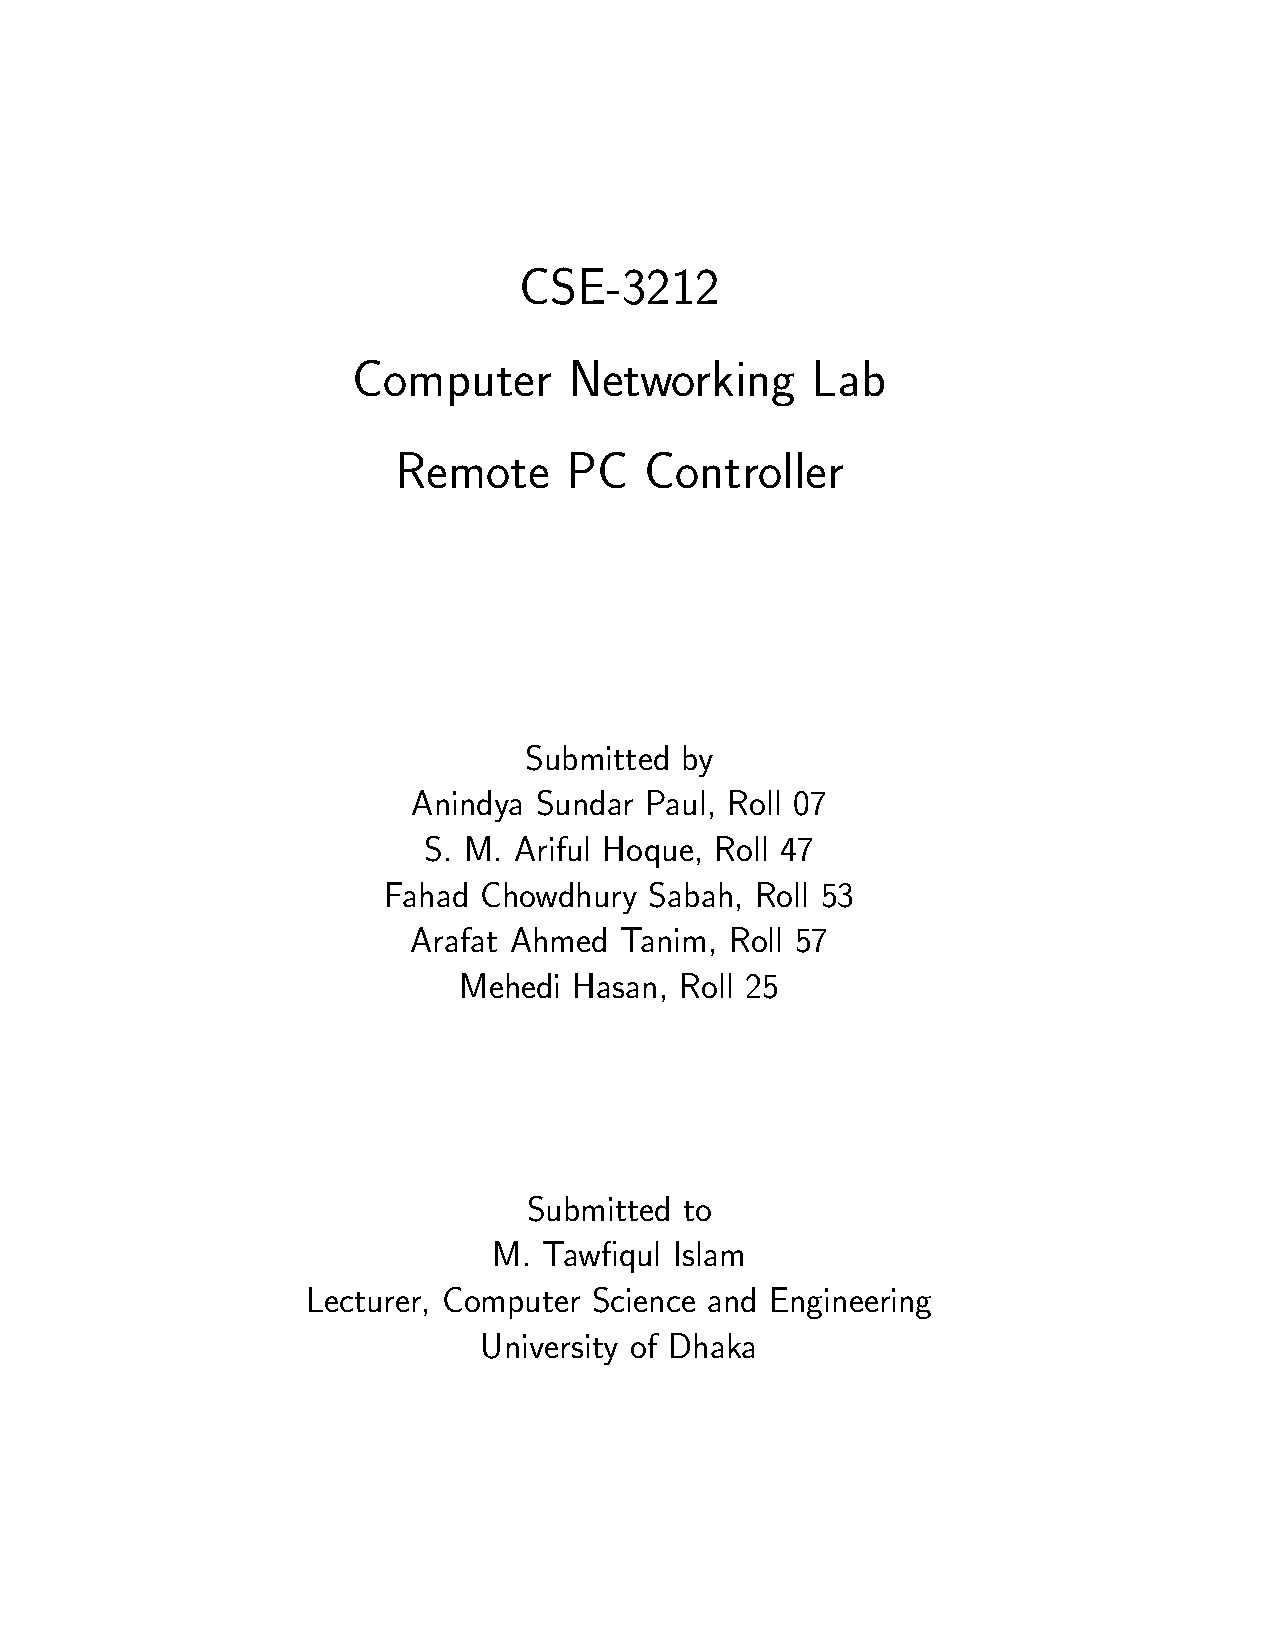
\includepdf{titlepage}
 
\pagenumbering{gobble}
 
\tableofcontents

\newpage

\pagenumbering{arabic}
 
\section{Introduction}

The project we will be working on is remote PC controller. The main idea of this project is to control a computer remotely by another computer. The computers will be connected through internet. We have to provide a solution that allows one user to control another user's pc remotely over internet.

\section{Motivation}

The concept of this project comes from the idea of solving a computer's problem remotely. It is an interesting project to work on as it not only solves a real world issue but also the idea of being able to computer another computer remotely is exciting. Through this project we will get a clear concept about TCP protocol, network programming, multi threading, screen sharing etc. Since this is a project for educational purpose, we have picked a standard software TeamViewer which is already available for real world problems. We look forward to make something similar.

\section{Project Details}

In this section we will be discussing the detailed functions of this project and how we will implement these functions.

\subsection{The Team}

Our team consists of five members.\\ \\
\textbf{Anindya Sundar Paul}: CEO.\\
\textbf{S. M. Ariful Hoque}: Back end developer.\\
\textbf{Fahad Chowdhury Sabah}: Front end developer.\\
\textbf{Mehedi Hasan}: Front end developer.\\
\textbf{Arafat Ahmed Tanim}: Front end developer.\\

\begin{figure}[h!]
\centering
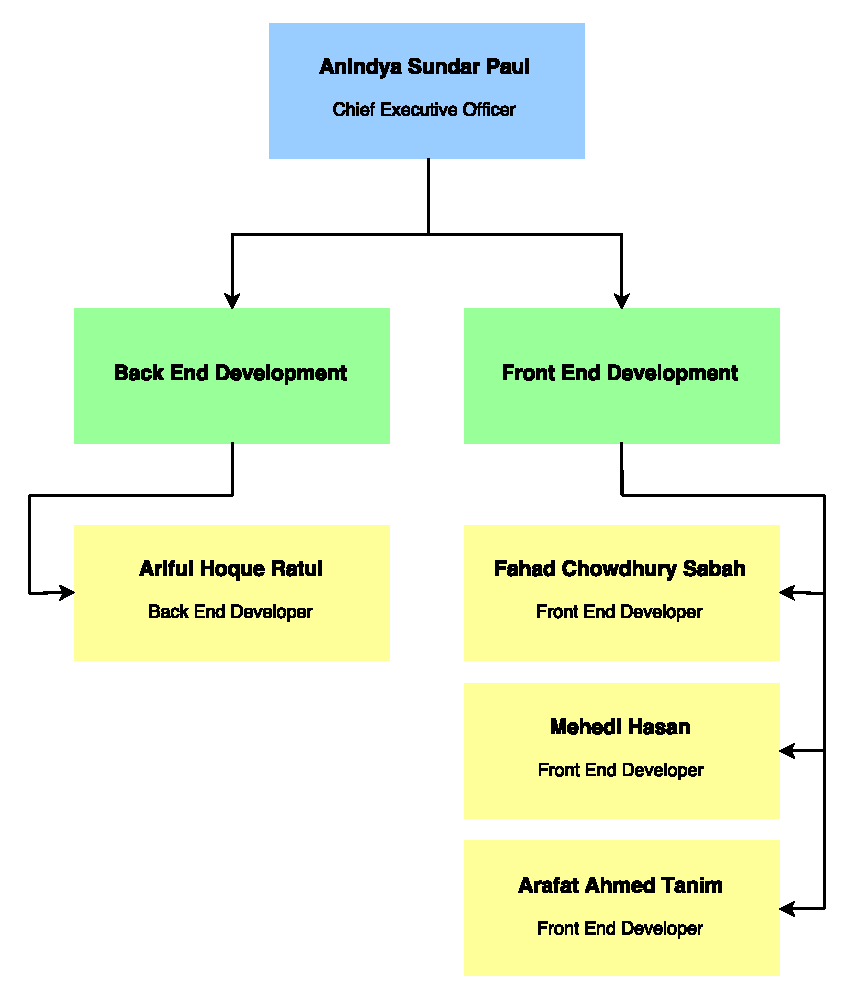
\includegraphics[scale=0.8]{remote-pc-controller-organogram}
\caption{Organogram}
\end{figure}

\textbf{Anindya Sundar Paul} will organize and supervise our project. He will also work as a backend developer. He will develop the basic algorithm to complete the project. The design of the user interface is also done by him. Finally he will assemble all into one piece of final solution.\\ \\

\textbf{S. M. Ariful Hoque} will work as a backend developer. He will do the core programming of the project. Based on the algorithm, he will develop the system using TCP protocol.\\ \\

\textbf{Fahad Chowdhury Sabah}, \textbf{Mehedi Hasan} and \textbf{Arafat Ahmed Tanim} will work as frontend developer. Based on the design, they will create the UI. Creating different buttons, windows, screens and making them functional is their primary job. They will use Java Swing library for this.\\ \\

Although the job is divided among all the members of the team, it is very much possible for one member to participate in another one's job.

\subsection{Use Case}

\begin{figure}[h!]
\centering
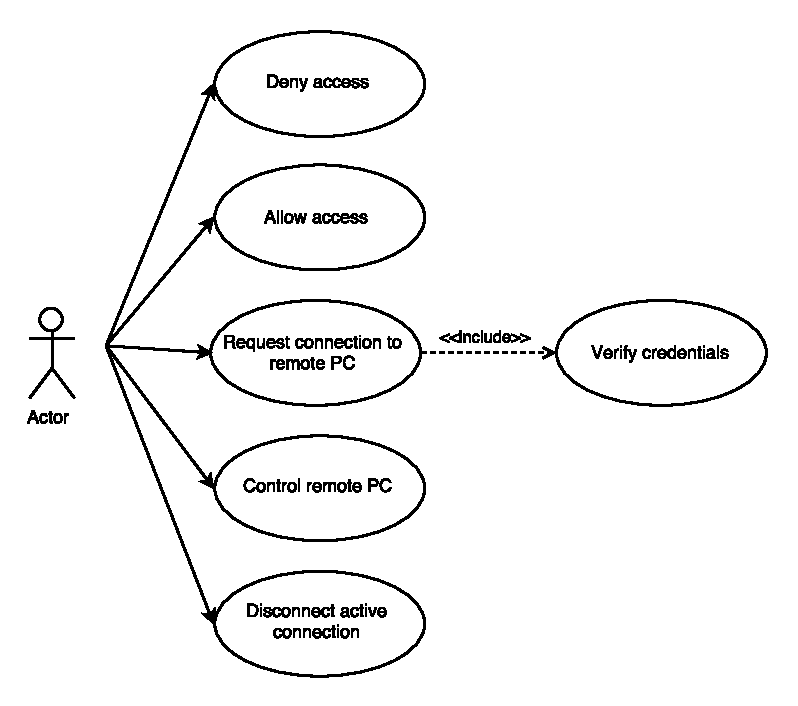
\includegraphics[scale=1]{remote-pc-controller-usecase}
\caption{Use Case Diagram}
\end{figure}

\newpage

\subsection{Workflow}

\begin{figure}[h!]
\centering
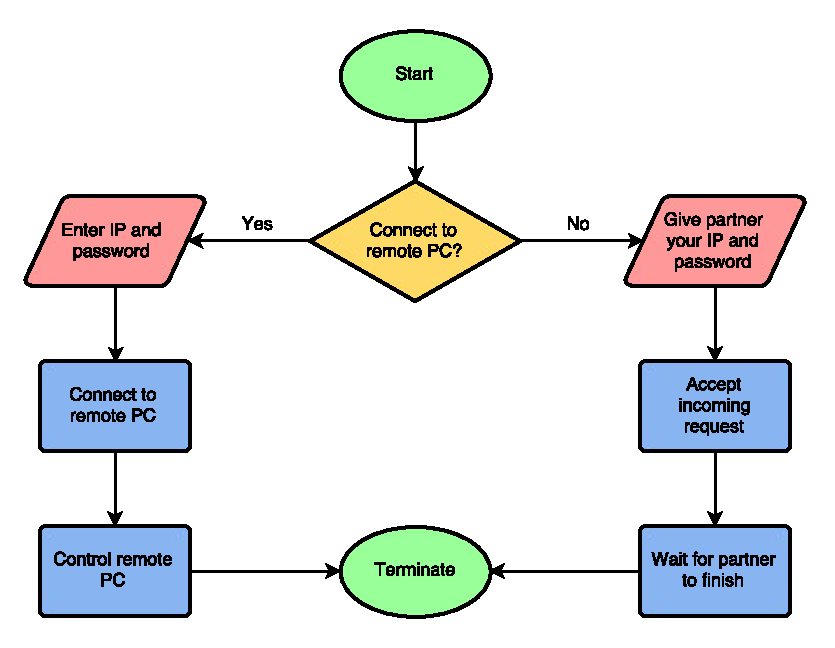
\includegraphics[scale=0.9]{remote-pc-controller-workflow}
\caption{Workflow Diagram}
\end{figure}

After starting the program, the user may act as controlled or controller. If the user wants to connect to remote PC and control it, he/she has to enter the IP and password provided by the remote PC. After entering valid IP and password the controller will send a request in order to have control. After accepting the request, the controller will have control of the remote PC. The remote PC user will also have access to his computer and may terminate at any point. After connecting to the remote PC, the controller will do his job and then terminate the program. \\
If the user wants his PC to be controlled, he/she will have to give his/her IP and password to the controller. This is a password generated for this sole program, not the master password. After getting the password and IP, the controller will send a request. If the remote PC user do not accept the request, the connection will not be made. If he/she accepts it, the controller will have control over the remote PC. The remote PC user may terminate the program at any moment.

\newpage

\subsection{User Interface}

We have tried our best to come up with a UI design so that the user can use the program very easily.

\subsubsection{Home}
When the software starts, the user will see this window. It provides the user with his own IP and password to share with another user. It also let's the user enter another user's IP and password in order to take control of the remote pc. Pressing the connect button will request access to the remote pc.

\begin{figure}[h!]
\centering
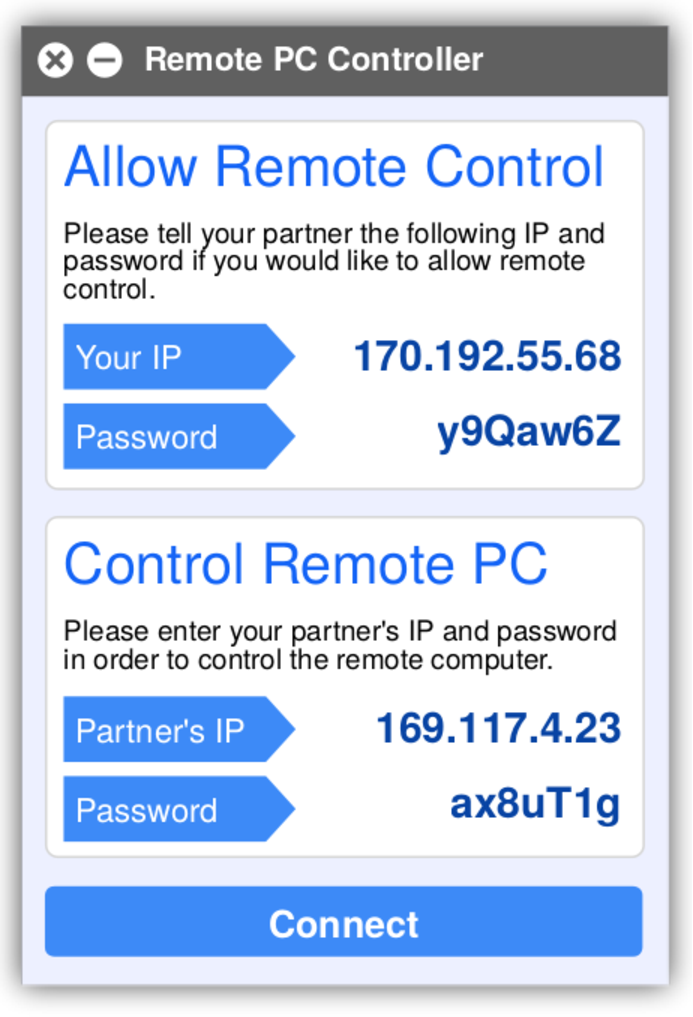
\includegraphics[scale=0.75]{home}
\caption{Home}
\end{figure}

\subsubsection{Incoming Request}
When any user receives request for access by his partner, this screen is shown. The user can chose to deny or allow access.

\begin{figure}[h!]
\centering
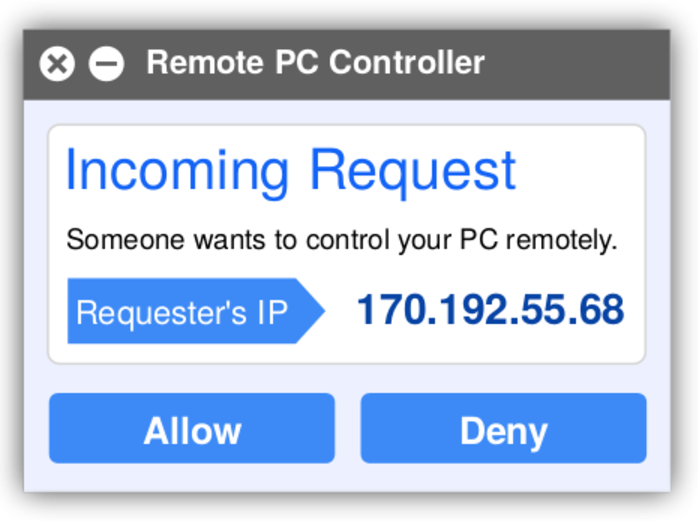
\includegraphics[scale=0.75]{incoming}
\caption{Incoming Request}
\end{figure}

\subsubsection{Connecting}
When the user tries to connect to a remote pc, this screen is shown while the program tries to connect to the remote pc in background.

\begin{figure}[h!]
\centering
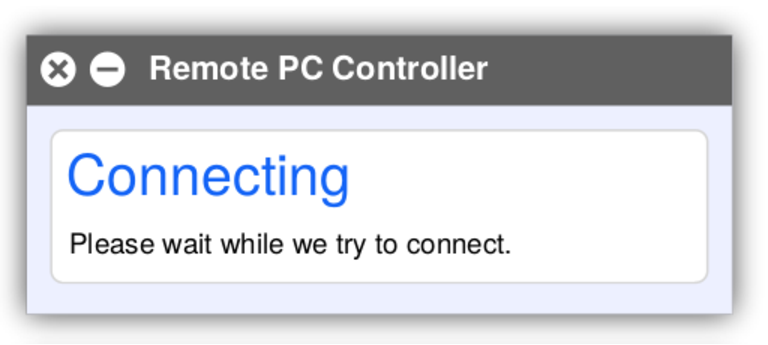
\includegraphics[scale=0.75]{connecting}
\caption{Connecting}
\end{figure}

\newpage

\subsubsection{Oops}
If the user enters wrong IP or password when trying to connect to partner, this screen is shown.

\begin{figure}[h!]
\centering
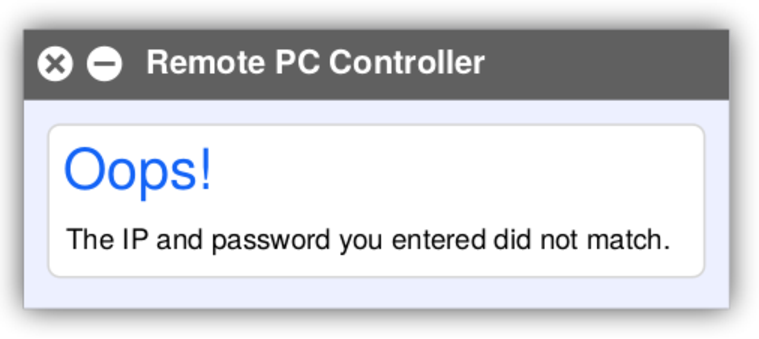
\includegraphics[scale=0.75]{oops}
\caption{Oops}
\end{figure}

\subsubsection{Denied}
If the remote user denies access to the user, this screen is shown.

\begin{figure}[h!]
\centering
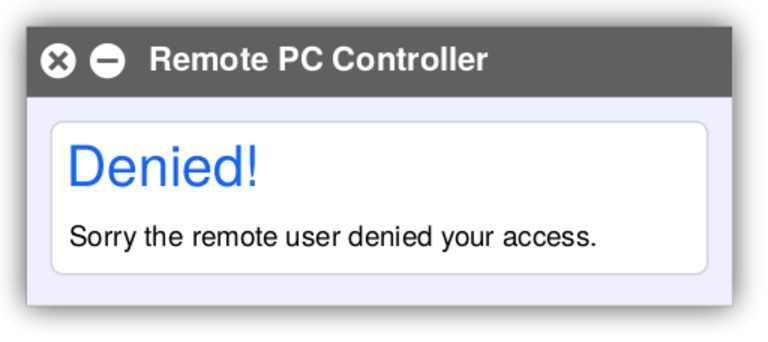
\includegraphics[scale=0.75]{denied}
\caption{Denied}
\end{figure}

\newpage

\subsubsection{Current Session}
If any successful connection gets established, the user being controlled is shown this screen through which he can choose to disconnect at any moment.

\begin{figure}[h!]
\centering
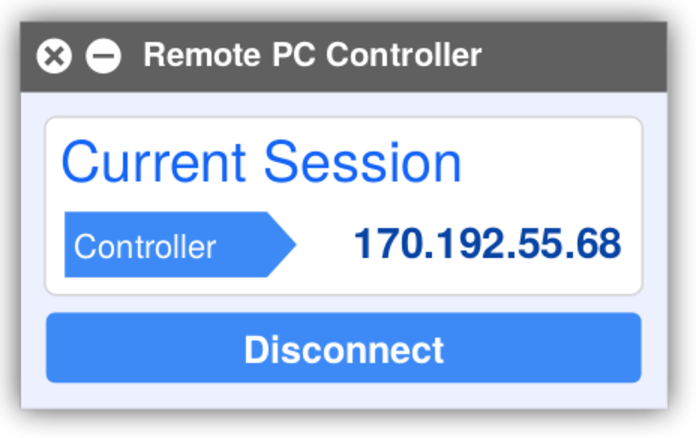
\includegraphics[scale=0.75]{current}
\caption{Current Session}
\end{figure}

\subsection{Implementation Approach}
The way we are planning on solving this problem is pretty straight forward. The program will create TCP connection between the two computers. As the connection gets established, two threads will be created for data transfer in two directions. Then the controller will receive screenshots of the remote pc continuously. As it gets screenshots, the user will use his mouse and keyboard and do what he wants to do. The mouse and keyboard events will be sent to the remote pc. Mouse cursor position will be calculated relative to the size of the screenshot thus resembling the proper position in the remote pc. As the remote pc receives the mouse and keyboard events, it will simulate those events. Thus we can control the pc remotely.

\newpage

\section{Our Goal}
Our main goal is to complete the basic project, which is to control a PC remotely through LAN by another PC. If it is completed before estimated time, we will try to implement some extensions.


\section{Conclusion}
Remote-PC-controller is a basic network programming project. This project will help us to have a better and clearer concept about different networking protocol and file transferring. Our goal is to complete this project within the fastest time and without any bug.

\end{document}
